
In this section, we present scalability results using a couple of test cases.  All the scalability experiments were performed 
on the {\it{Jaguar}} supercomputer at Oak Ridge National Laboratory (ORNL). The architectural details for this supercomputer
 can be found in \cite{jaguar}. The code is written in the C++ language and built on top of \texttt{PETSc} and \texttt{DENDRO} packages. 
 Specifically, we use \texttt{DENDRO} for managing linear octrees and \texttt{PETSc} for managing distributed regular grids and profiling. 

{\em Example 1.} In this example, we consider a uniform tensor-product grid obtained by using Gaussian quadrature rule to
 compute (\ref{heat}) within the unit cube. The source strength $f(y)$ is chosen randomly and the targets are same as the
  sources. We used our expansion algorithm and incorporated the acceleration techniques
  introduced in \cite{fggt} for tensor-product grids. They are based on {\em separation of variables} and
  the complexity of the S2W and L2T steps is reduced from $\bigO(p^3 N)$ to $\bigO(p N)$. 

We report the weak scalability results in Figure \ref{f:isoUniform}. The grain size is fixed to approximately 30 million 
sources/targets per CPU. We also reduce $\delta$ so that the number of FGT boxes per CPU remains fixed. We get excellent
 scalabilty in this case--only a small increase in timing as we go from 1 to 4096 CPUs. This is  because the cost is dominated 
 by the S2W and L2T steps and both of them are embarassingly parallel in our implementation. There is only one communication 
 step in the algorithm: a point-to-point communication in the W2L step for communicating the plane-wave expansions of ghost boxes.

\begin{figure}
	\begin{center}
	
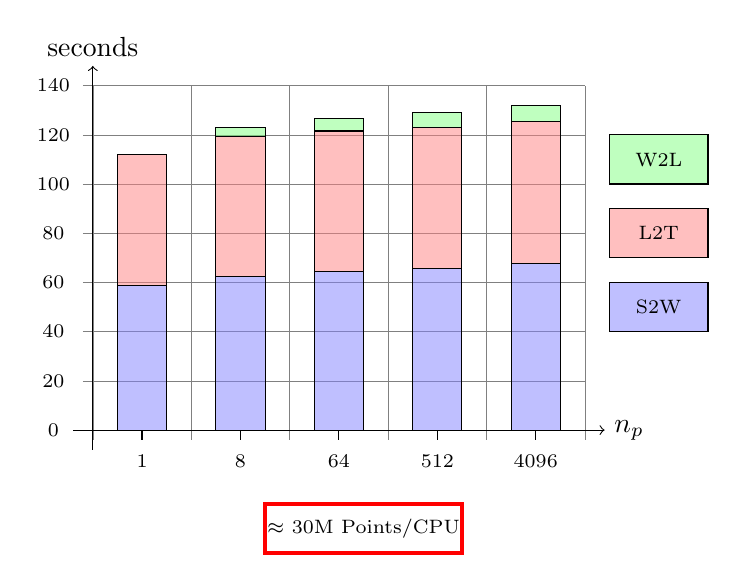
\begin{tikzpicture}[scale=1.25]

\draw[very thin, color=gray, xstep=1, ystep=0.5] (-0.1,-0.1) grid (5, 3.5);
\draw[->] (-0.2, 0) -- (5.2, 0) node[right] {$n_p$};
\draw[->] (0, -0.2) -- (0, 3.7) node[above] {seconds};

\newdimen\yscale

\yscale= 0.025 cm

\foreach \pos/\label in {0.5/1, 1.5/8, 2.5/64, 3.5/512, 4.5/4096} {
\draw (\pos,0) -- (\pos,-0.1) (\pos cm,-2.5ex) node [anchor=base,fill=white,inner sep=1pt]  {\scriptsize{\label}};
}

\foreach \label in {0, 20, ..., 140} {
 \draw (-0.4, \label\yscale) node {\scriptsize{\label}};
}

\draw[fill=blue!50, fill opacity=0.5] (4.5, 2.25) ++ (0.75, -1.25) rectangle +(1.0, 0.5);
\draw (4.5, 2.25) ++ (1.25, -1.0) node {\scriptsize{S2W}};

\draw[fill=red!50, fill opacity=0.5] (4.5, 1.75) ++ (0.75, 0.0) rectangle +(1.0, 0.5);
\draw (4.5, 1.75) ++ (1.25, 0.25) node {\scriptsize{L2T}};

\draw[fill=green!50, fill opacity=0.5] (4.5, 1.25) ++ (0.75, 1.25) rectangle +(1.0, 0.5);
\draw (4.5, 1.25) ++ (1.25, 1.5) node {\scriptsize{W2L}};

\draw[red, ultra thick] (1.75, -1.25) rectangle +(2.0, 0.5);
\draw (2.75, -1.0) node {\scriptsize{$\approx$ 30M Points/CPU}};

\newdimen\mypos
\newdimen\myoff

\foreach \pos/\vala/\valb/\valc/\vald/\vale/\valf in { 
0/58.75/53.36/0.0698/112.19/29.2M/$\frac{1}{16}$,
1/62.25/56.98/3.90/120.93/233.8M/$\frac{1}{64}$,
2/64.39/57.18/4.93/125.06/1.9B/$\frac{1}{256}$,
3/65.56/57.50/5.92/127.62/15.0B/$\frac{1}{1024}$,
4/67.53/57.75/6.59/131.65/119.7B/$\frac{1}{4096}$ } { 

\mypos=\pos cm
\advance \mypos by 0.5 cm

\advance \mypos by -0.25 cm

\myoff=0 cm

\draw[fill=blue!50, fill opacity=0.5] (\mypos, \myoff) rectangle +(0.5, \vala\yscale);
\advance \myoff by \vala\yscale

\draw[fill=red!50, fill opacity=0.5] (\mypos, \myoff) rectangle +(0.5, \valb\yscale);
\advance \myoff by \valb\yscale

\draw[fill=green!50, fill opacity=0.5] (\mypos, \myoff) rectangle +(0.5, \valc\yscale);

}

\end{tikzpicture}


	\end{center}
\caption{\label{f:isoUniform} Isogranular scalability for an uniform point distribution. For
 this experiment, we set $\epsilon = 10^{-6}$. The reported times for 
each component are the maximum values for that component across all the processors. The total wall-clock
time is reported in bold face.} 
\end{figure}

{\em Example 2.} In this example, we consider a Gaussian random distribution of points in the unit cube. We construct
a linear octree from these points such that each leaf contains $7^3$ sources/targets within it. We used 
 our octree-based FGT algorithm. We present the weak scalability results in Figure \ref{f:isoGaussian}. We varied the
 number of input points such that the number of expand leaves per CPU and the number of direct leaves per CPU remain
  approximately constant as we vary the number of CPUs. There is a significant increase in the timings between the 
  1 CPU and 8 CPU cases because there were no direct leaves for the 1 CPU case. Otherwise, the scalability is very good.

Note that the timings in the nonuniform case have increased considerably compared to the uniform case (Figure \ref{f:isoUniform}). A 
major factor is that the point distribution is random and we cannot use the tensor-product acceleration in the current example. However,
 there are a few other accelerations that we have not incorporated, we list them below.
%
\begin{itemize}
  \item In \cite{fggt}, it is noted that a Hermite expansion is much more effective in condensing the source information than a plane-wave
   expansion. In the S2W step, significant computational speedup can be achieved by first forming the Hermite expansion and then converting 
   it to a plane-wave expansion using the scheme proposed in \cite{fggt}. Similary, in the L2T step, instead of directly evaluating the 
   local plane-wave expansion, it is beneficial to first convert the local plane-wave expansion into a local Taylor expansion and then evaluate 
   the Taylor expansion at the targets. 
  \item In this example, we have set $c = 1$. From Figure \ref{f:isoGaussian}, it is clear that the tree $T_d$ is taking disproportionately 
  more time than $T_e$. There exists an optimal value for the $c$ depending on the free parameters $m$, $\delta$ and $\epsilon$, below which
 the timings are higher because of higher cost for the truncation algorithm and above which, the timings are higher because
 there will be fewer points for FGT box. However, we did not compute this optimal value for this experiment; our choice of $c$ for this experiment
 was rather arbitrary.
\end{itemize}
%
We will include these accelerations in our final submission. 

\begin{figure}
	\begin{center}
	
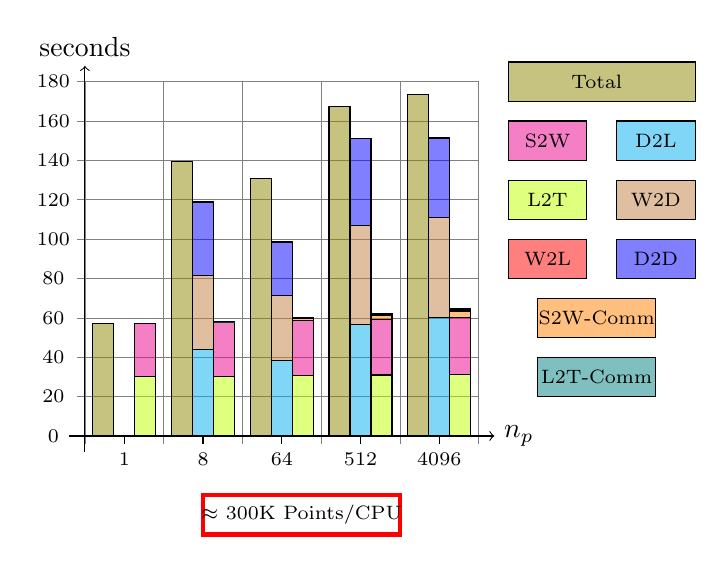
\begin{tikzpicture}[scale=1.0]

\draw[very thin, color=gray, xstep=1, ystep=0.5] (-0.1,-0.1) grid (5, 4.5);
\draw[->] (-0.2, 0) -- (5.2, 0) node[right] {$n_p$};
\draw[->] (0, -0.2) -- (0, 4.7) node[above] {seconds};

\newdimen\yscale

\yscale= 0.025 cm

\foreach \pos/\label in {0.5/1, 1.5/8, 2.5/64, 3.5/512, 4.5/4096} {
\draw (\pos,0) -- (\pos,-0.1) (\pos cm,-2.5ex) node [anchor=base,fill=white,inner sep=1pt]  {\scriptsize{\label}};
}

\foreach \label in {0, 20, ..., 180} {
 \draw (-0.4, \label\yscale) node {\scriptsize{\label}};
}


\draw[fill=olive, fill opacity=0.5] (5.375, 4.25) rectangle +(2.375, 0.5);
\draw (6.5, 4.5) node {\scriptsize{Total}};

\draw[fill=magenta, fill opacity=0.5] (5.375, 3.5) rectangle +(1.0, 0.5);
\draw (5.875, 3.75) node {\scriptsize{S2W}};

\draw[fill=lime, fill opacity=0.5] (5.375, 2.75) rectangle +(1.0, 0.5);
\draw (5.875, 3.0) node {\scriptsize{L2T}};

\draw[fill=red, fill opacity=0.5] (5.375, 2.0) rectangle +(1.0, 0.5);
\draw (5.875, 2.25) node {\scriptsize{W2L}};

\draw[fill=cyan, fill opacity=0.5] (6.75, 3.5) rectangle +(1.0, 0.5);
\draw (7.25, 3.75) node {\scriptsize{D2L}};

\draw[fill=brown, fill opacity=0.5] (6.75, 2.75) rectangle +(1.0, 0.5);
\draw (7.25, 3.0) node {\scriptsize{W2D}};

\draw[fill=blue, fill opacity=0.5] (6.75, 2.0) rectangle +(1.0, 0.5);
\draw (7.25, 2.25) node {\scriptsize{D2D}};

\draw[fill=orange, fill opacity=0.5] (5.75, 1.25) rectangle +(1.5, 0.5);
\draw (6.5, 1.5) node {\scriptsize{S2W-Comm}};

\draw[fill=teal, fill opacity=0.5] (5.75, 0.5) rectangle +(1.5, 0.5);
\draw (6.5, 0.75) node {\scriptsize{L2T-Comm}};

\draw[red, ultra thick] (1.5, -1.25) rectangle +(2.5, 0.5);
\draw (2.75, -1.0) node {\scriptsize{$\approx$ 300K Points/CPU}};


\newdimen\mypos
\newdimen\myoff

\foreach \pos/\vala/\valb/\valc/\vald/\vale/\valf/\valg/\valh/\vali/\valj/\valk/\vall/\valm in {
 0/0/0/0/30.07/27.18/0.0094/0.0045/0.014/57.28/827/0/283.7K/$\frac{1}{16}$,
 1/43.93/37.48/37.46/30.27/27.37/0.426/0.014/0.143/139.4/6666/6/2.3M/$\frac{1}{64}$,
 2/38.37/32.88/27.31/30.86/27.78/1.03/0.052/0.34/130.7/53929/126/18.5M/$\frac{1}{256}$,
 3/56.84/50.16/44.36/30.97/28.41/1.99/0.187/0.471/167.36/433226/880/148.9M/$\frac{1}{1024}$,
 4/60.18/50.65/40.56/31.08/29.24/3.18/0.567/0.924/173.42/3474244/7837/1.2B/$\frac{1}{4096}$
  } { 

\mypos=\pos cm
\advance \mypos by 0.5 cm

\advance \mypos by -0.4 cm
\myoff=0 cm

%Total

\draw[fill=olive, fill opacity=0.5] (\mypos, \myoff) rectangle +(0.266667, \vali\yscale);

%Direct

\advance \mypos by 0.266667 cm

\myoff=0 cm

\draw[fill=cyan, fill opacity=0.5] (\mypos, \myoff) rectangle +(0.266667, \vala\yscale);
\advance \myoff by \vala\yscale

\draw[fill=brown, fill opacity=0.5] (\mypos, \myoff) rectangle +(0.266667, \valb\yscale);
\advance \myoff by \valb\yscale

\draw[fill=blue, fill opacity=0.5] (\mypos, \myoff) rectangle +(0.266667, \valc\yscale);

%Expand

\advance \mypos by 0.266667 cm

\myoff=0 cm

\draw[fill=lime, fill opacity=0.5] (\mypos, \myoff) rectangle +(0.266667, \vald\yscale);
\advance \myoff by \vald\yscale

\draw[fill=magenta, fill opacity=0.5] (\mypos, \myoff) rectangle +(0.266667, \vale\yscale);
\advance \myoff by \vale\yscale

\draw[fill=orange, fill opacity=0.5] (\mypos, \myoff) rectangle +(0.266667, \valf\yscale);
\advance \myoff by \valf\yscale

\draw[fill=teal, fill opacity=0.5] (\mypos, \myoff) rectangle +(0.266667, \valg\yscale);
\advance \myoff by \valg\yscale

\draw[fill=red, fill opacity=0.5] (\mypos, \myoff) rectangle +(0.266667, \valh\yscale);

}

\end{tikzpicture}


	\end{center}
\caption{\label{f:isoGaussian} Isogranular scalability for a gaussian point distribution. For
 this experiment, we set $\epsilon = 10^{-3}$. The reported times for each component are the
 maximum values for that component across all the processors. The total wall-clock
time is reported in bold face.} 
\end{figure}
